\chapter{VisTex：面向目标级视觉语言模型的视觉文本化图像提示}

\section{研究背景与问题提出}
目标检测方法通常依赖大规模标注数据\cite{redmon2016you,ren2016faster}，在稀缺场景（如长尾类别、专业领域与医学影像）中往往难以获取足够标注。因此，少样本目标检测（Few-shot Object Detection, FSOD）\cite{wang2019metadet,Qiao_2021_defrcn2}成为重要研究方向。近年来，视觉语言预训练模型（VLMs）通过海量图文对学习具有较强泛化能力的跨模态表示，使得“以文本提示进行零样本迁移”成为可能。然而，医学图像与专业领域的下游任务仍存在三类典型困难：其一，下游类别在预训练语料中覆盖不足；其二，文本提示的描述粒度有限，容易产生语义偏置与遗漏；其三，细粒度目标往往共享相近的文本描述，仅靠文本难以区分\cite{xu2023mqdet,du2022learning}。

目标级视觉语言模型（Object-level Vision-Language Models, OVLMs）\cite{li2022glip,dou2022fiber,liu2023groundingdino}以 GLIP\cite{li2022glip} 为代表，利用 grounding 数据与多尺度/多阶段跨注意力结构建立了更强的\textbf{目标级图文对齐}，在零样本检测中显著优于 CLIP\cite{radford2021clip} 等图像级 VLM。然而，如何在\textbf{不破坏 OVLM 预训练的图文对齐}前提下，把下游任务中少量支持样本（support images）所包含的视觉语义注入到提示推理过程，仍然是一个关键难题。

\section{动机：引入下游视觉语义而不破坏图文对齐}
现有基于 VLM 的 FSOD 方法通常通过\textbf{微调原模型权重}或\textbf{引入额外可学习结构}来利用支持图像信息，但在少量目标域数据下，这两类做法都可能导致原有的目标--文本相似度分布发生偏移，从而损害源域对齐并削弱泛化能力。更进一步地，许多 OVLM（如 GLIP 与 GroundingDINO）本质上是\textbf{“仅支持文本提示”的模型}，由于结构设计限制，缺少对图像提示（image prompting）的原生支持\cite{li2022glip,liu2023groundingdino}。

图像提示为解决上述问题提供了一条思路：用支持图像作为提示，与文本提示一起为下游推理提供语义引导\cite{luddecke2022clipseg,xu2023mqdet}。然而，现有代表方法 MQ-Det\cite{xu2023mqdet} 通过在文本编码器内部额外引入可学习跨注意力模块来实现“图像调制文本”，它主要对现有文本 token 进行重加权，而非直接引入新的视觉信息；同时，新引入的结构也可能进一步偏置 OVLM 的预训练对齐。

基于此，本章提出 VisTex-OVLM：通过\textbf{视觉文本化（visual textualization）}将支持图像投影到 OVLM 的\textbf{文本特征空间}，把支持样本以“文本 token”的形式直接并入提示序列，从而在不修改 OVLM 主体结构的前提下实现\textbf{直接图像提示}。

\section{任务定义与符号说明}
在经典 FSOD 设置中，存在基类数据集 $D_b$（类别集合 $C_b$）与新类数据集 $D_n$（类别集合 $C_n$），满足 $C_b\cap C_n=\emptyset$。在新类集合中，每个类别仅提供至多 $K$ 个带框标注实例（$K$-shot）。测试阶段中，提供少量标注的图像称为支持图像（support images），待预测的图像称为查询图像（query images）。在更一般的 GFSOD 设置中，测试类别集合为 $C_b\cup C_n$，要求模型在新类上提升的同时保持基类性能。

对 OVLM 的多尺度/多阶段编码过程，记第 $i$ 个 stage 的中间视觉特征与文本特征分别为 $R^i$ 与 $P^i$，其中 $i=0,1,\ldots,L$。多尺度特征记为 $R^i=\left[R^{i,(j)}\right]_{j=0}^{M-1}$，其中 $M$ 表示尺度数。

\section{方法：VisTex-OVLM 视觉文本化框架}
图 \ref{fig:vistex_framework} 给出了 VisTex-OVLM 的整体流程。其核心由两部分组成：\textbf{多尺度视觉文本化模块（Multi-scale Textualizing Blocks, MSTB）}与\textbf{多阶段融合策略（Multi-stage Fusion, MSF）}。二者共同将支持图像映射为一个或多个\textbf{视觉文本化 token}，并与常规文本提示 token 拼接后直接输入\textbf{冻结的} OVLM，实现无需改动主干结构的图像提示推理。

\begin{figure}[t]
  \centering
  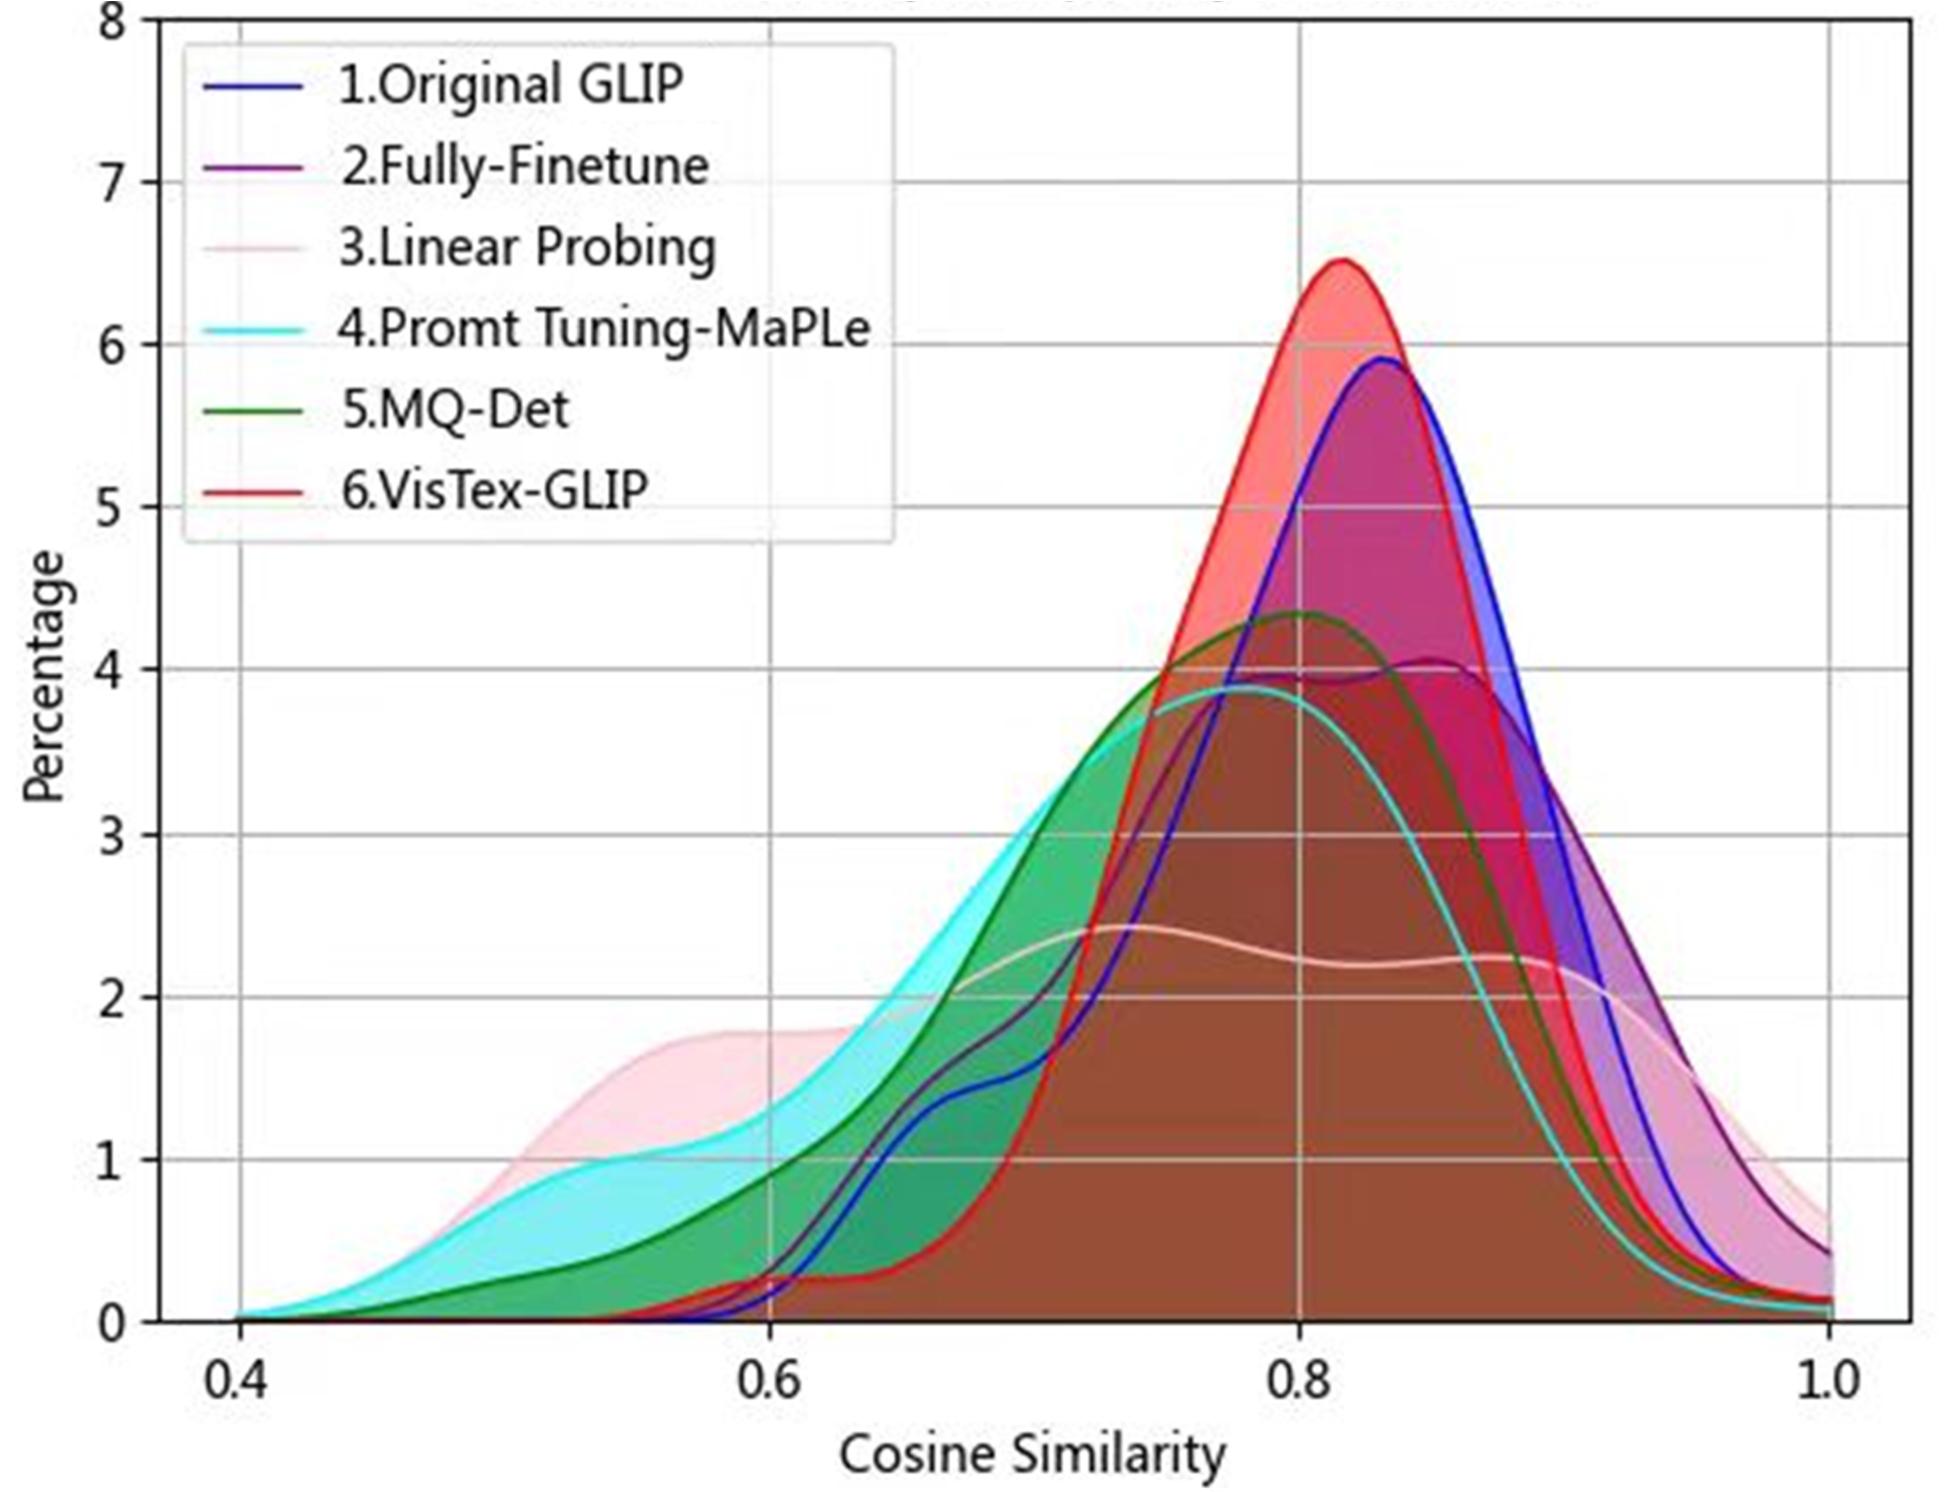
\includegraphics[width=0.96\linewidth]{chapters/PAPERS/VisTex_ICCV_ver/cosine1.png}
  \caption{不同迁移方式对 OVLM 源域图文对齐的影响。在有限目标域数据下，结构或权重的修改会使源域 object--text 相似度分布发生偏移，从而部分破坏预训练对齐。}
  \label{fig:vistex_cosine}
\end{figure}

\begin{figure}[t]
  \centering
  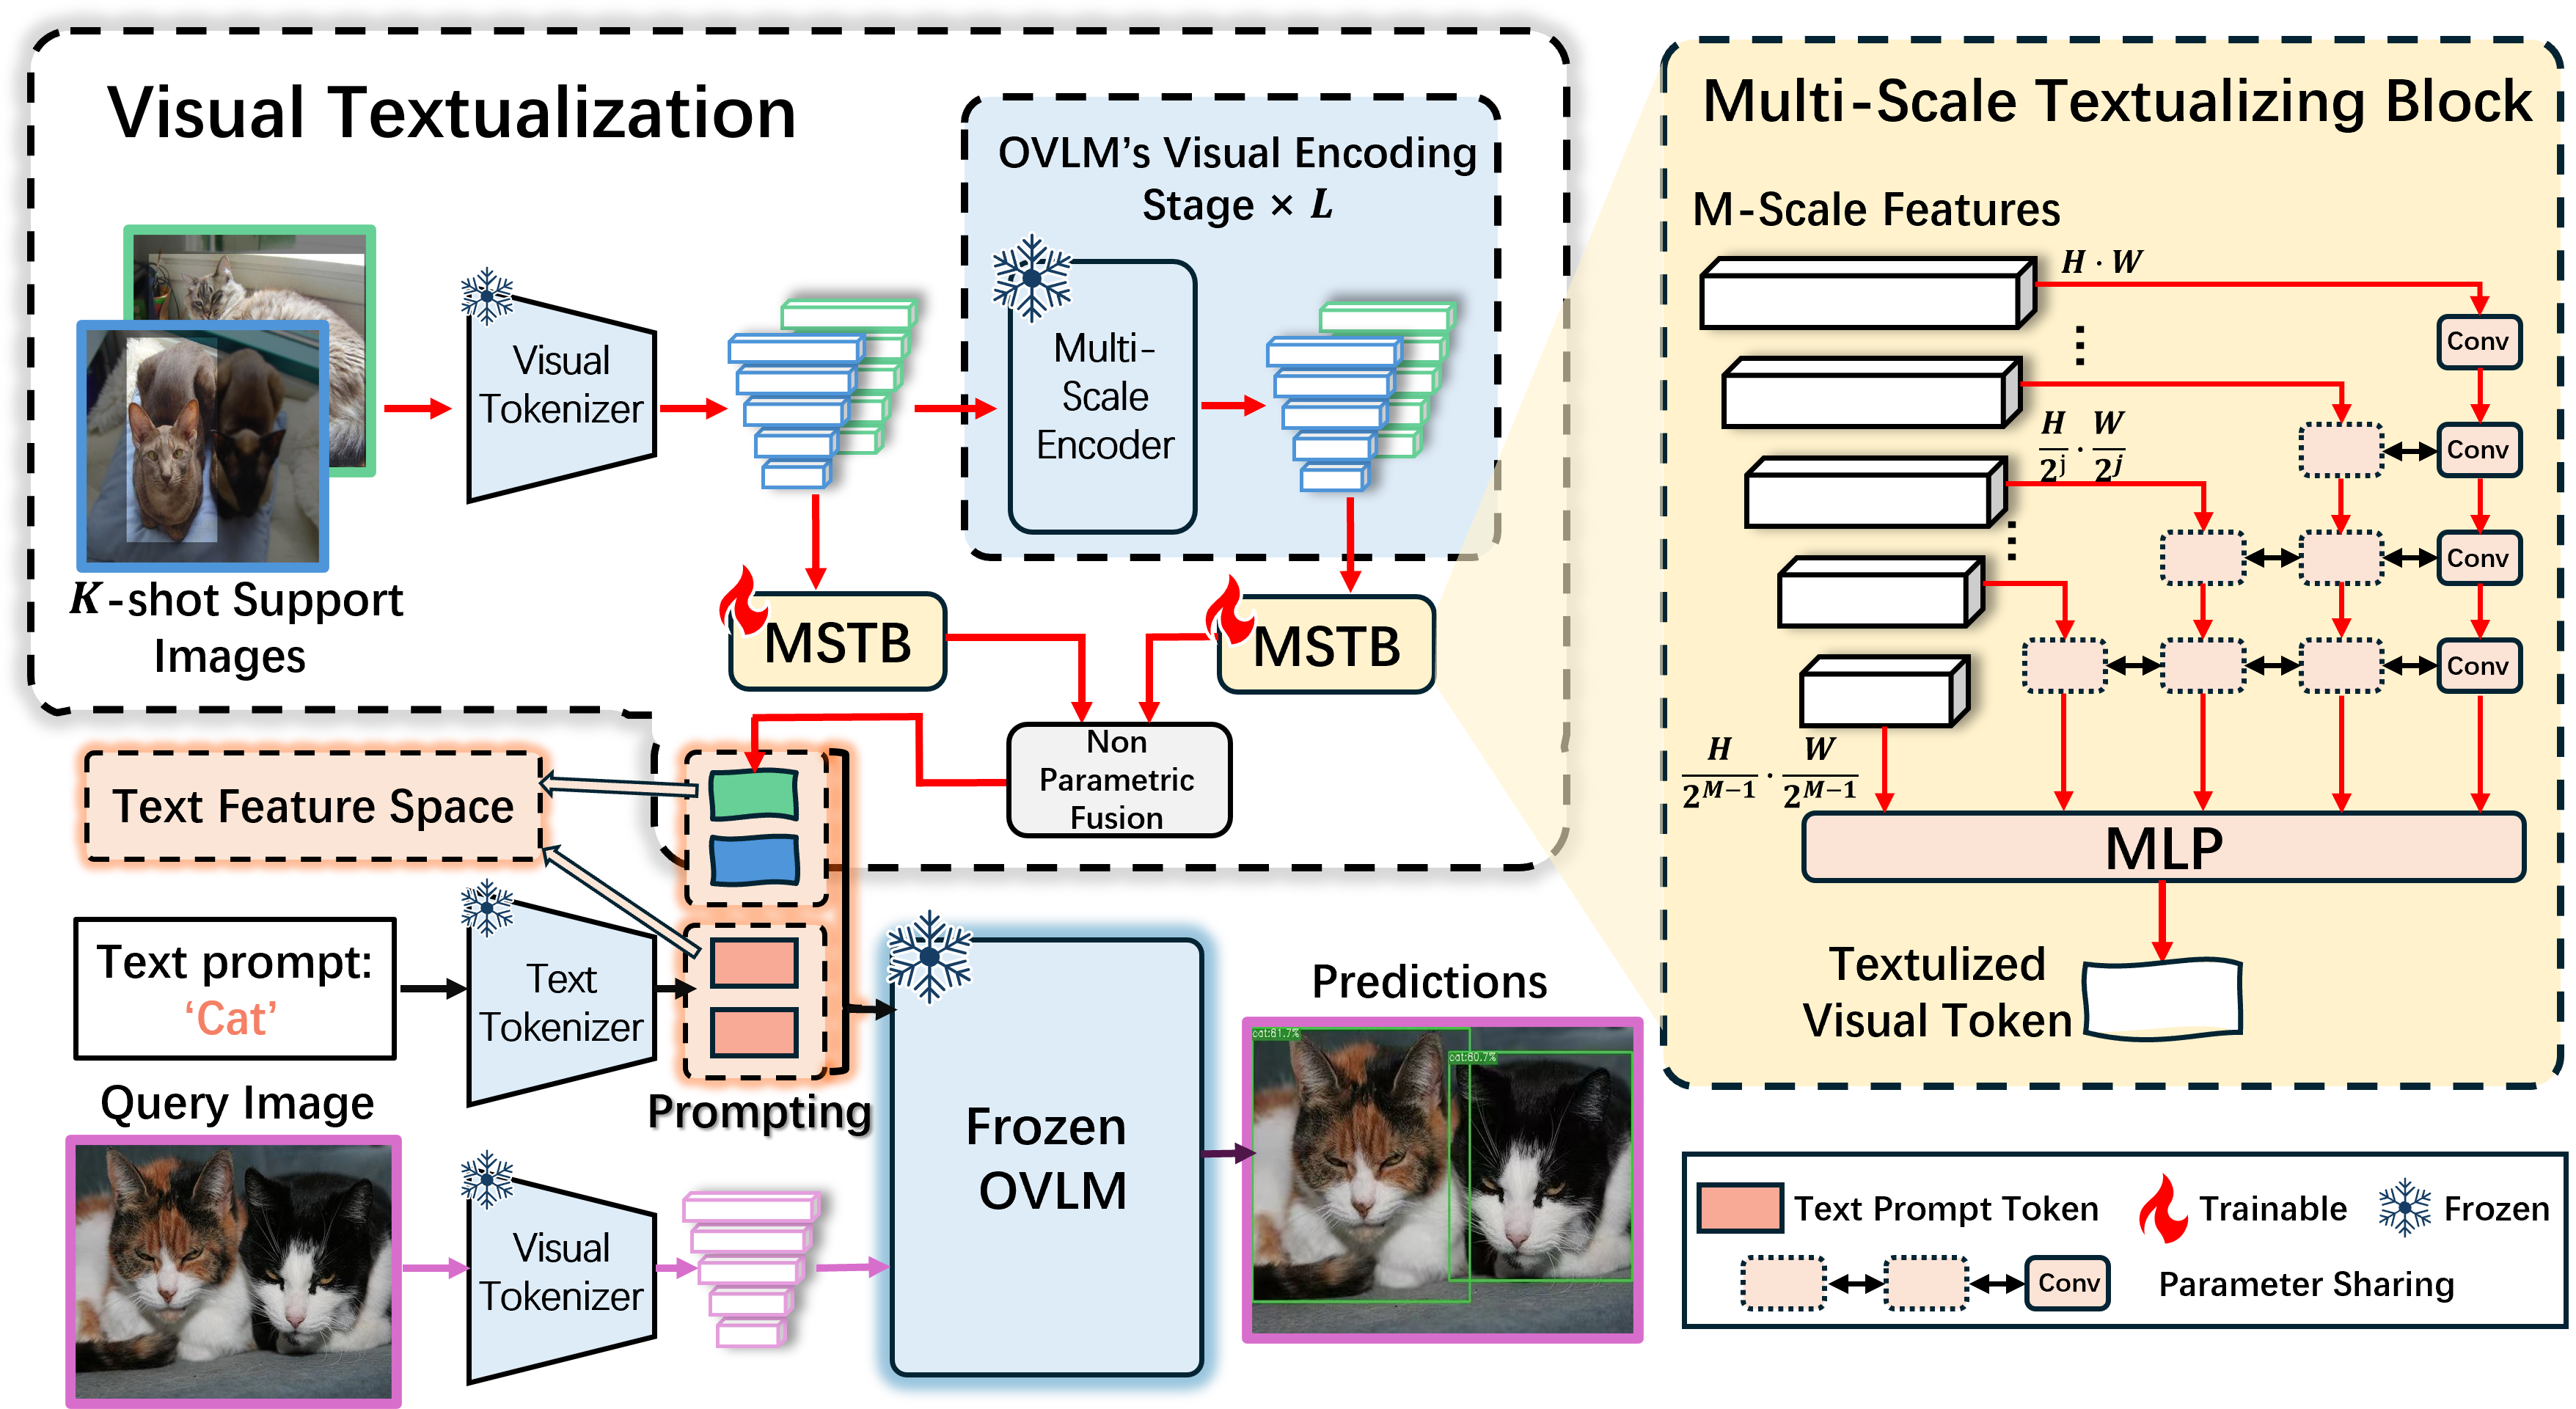
\includegraphics[width=\linewidth]{chapters/PAPERS/VisTex_ICCV_ver/method.png}
  \caption{VisTex-OVLM 框架示意。通过 MSTB 与 MSF 将支持图像投影到 OVLM 的文本特征空间，生成视觉文本化 token，并与文本提示共同驱动未修改的 OVLM（如 GLIP\cite{li2022glip}、GroundingDINO\cite{liu2023groundingdino}）完成少样本检测。}
  \label{fig:vistex_framework}
\end{figure}

\subsection{图像提示工程（Image Prompt Engineering）}
由于检测属于密集预测任务，支持图像中同时包含目标、背景及其它干扰物体。为最大化利用少样本标注，本章采用图像提示工程：结合支持图像中的目标框信息，对框外区域进行模糊化处理，使得支持图像更聚焦于目标实例\cite{luddecke2022clipseg}。

\subsection{多尺度视觉文本化（MSTB）}
给定提示工程后的支持图像 $x_S$，使用冻结的 OVLM 视觉编码器提取各 stage 的多尺度特征 $R^i_S=\left[R_S^{i,(j)}\right]_{j=0}^{M-1}$。MSTB 的目标是将不同尺度的视觉特征统一聚合，并映射到文本特征维度，从而得到 stage 级的视觉文本化特征 $\widetilde{P^i_S}$。

为高效共享跨尺度知识并降低训练成本，MSTB 采用参数共享策略：对除最小尺度以外的各尺度特征使用共享的下采样卷积逐级压缩到同一空间分辨率，拼接后再用 MLP 映射到文本空间，形式化为：
\begin{equation}
\begin{aligned}
    \widetilde{R^{i,(j)}_S} = \left\{
    \begin{array}{ll}
    \left( \prod_{j}^{M-2} \operatorname{Conv}_{\text{down}}^{i,(j)}\right) \left( R^{i,(j)}_S \right), & \text{if } j \neq M-1 \\
    R^{i,(j)}_S, & \text{if } j = M-1
    \end{array}
    \right.
\end{aligned}
\label{eq:vistex_downsample}
\end{equation}
\begin{equation}
    \widetilde{R^i_S} = \left[ \widetilde{R^{i,(j)}_S} \right]_{j=0}^{M-1},
\label{eq:vistex_concat}
\end{equation}
\begin{equation}
    \widetilde{P^i_S} = \operatorname{MLP}^i \left( \widetilde{R^i_S} \right).
\label{eq:vistex_mlp}
\end{equation}

\subsection{多阶段融合（MSF）}
OVLM 的多阶段编码对应着多阶段的跨模态对齐过程。为充分利用这种对齐先验，本章进一步对各 stage 的 $\widetilde{P^i_S}$ 进行非参数融合，得到最终的视觉文本化 token $\widetilde{P_S}$：
\begin{equation}
    \widetilde{P_S} = \operatorname{MSF} \left( \{ \widetilde{P^i_S}\}_{i=0}^L \right).
\label{eq:vistex_msf}
\end{equation}
由于 MSF 采用非参数操作（如跨 stage 的 max pooling），因此在不引入额外参数的情况下即可利用 OVLM 的多阶段对齐能力。

\subsection{直接支持图像提示（Direct Image Prompting）}
得到 $\widetilde{P_S}$ 后，将其与文本提示 $t$ 经 BERT 编码得到的 token 直接拼接，构成输入 OVLM 的提示序列：
\begin{equation}
    P^0 = \left[ \operatorname{BERT}\left(t\right), \widetilde{P_S} \right].
\label{eq:vistex_prompt_1shot}
\end{equation}
对于 $K$-shot 设置，为保持每个 shot 的独立性，直接拼接多个视觉文本化 token：
\begin{equation}
    P^0 = \left[ \operatorname{BERT}\left(t\right), \widetilde{P_{S_1}}, \cdots, \widetilde{P_{S_K}} \right].
\label{eq:vistex_prompt_kshot}
\end{equation}
在训练阶段，仅更新 MSTB 的参数，OVLM 主体保持冻结；训练完成后，MSTB 可直接对新类支持样本进行视觉文本化，从而在不微调 OVLM 的条件下完成少样本检测。

\section{实验设置与结果分析}
本章遵循标准 FSOD 协议\cite{wang2020frustratingly,zhang2022metaDETR1}在 PASCAL VOC\cite{everingham2010pascalvoc} 与 MSCOCO\cite{lin2014microsoftCOCO} 上评估方法，并进一步在 LVIS\cite{gupta2019lvis}、ODinW\cite{li2022odinw} 以及多个医学数据集（如 MoNuSeg\cite{kumar2017dataset}、CoNSeP\cite{graham2019hover} 等）上验证开放集迁移能力。
（1）\textbf{标准 FSOD/GFSOD 基准。} VisTex-OVLM 在 PASCAL VOC 与 MSCOCO 的多种 shot 设置下取得了显著提升，并在兼顾 base/novel 类别的 GFSOD 设置中保持了对基类的稳定识别能力。为便于在学位论文中呈现关键结论，这里给出 GFSOD 代表性结果（MSCOCO 10-shot/30-shot）。

\begin{table}[t]
    \centering
    \resizebox{0.8\linewidth}{!}{
    \begin{tabular}{ccccccc}
    \hline
    \multicolumn{1}{c|}{} & \multicolumn{3}{c|}{\textbf{10-shot}} & \multicolumn{3}{c}{\textbf{30-shot}} \\ \cline{2-7} 
    \multicolumn{1}{c|}{\multirow{-2}{*}{\textbf{Method}}} & \textbf{AP} & \textbf{bAP} & \multicolumn{1}{c|}{\textbf{nAP}} & \textbf{AP} & \textbf{bAP} & \textbf{nAP} \\ \hline
    \multicolumn{7}{c}{\textbf{non-VLM-based}} \\ \hline
    \multicolumn{1}{c|}{\textbf{DiGeo \cite{ma2023digeo}}} & 32.0 & 39.2 & \multicolumn{1}{c|}{10.3} & 33.1 & 39.4 & 14.2 \\
    \multicolumn{1}{c|}{\textbf{DE-VIT-L \cite{zhang2023devit}}} & 30.6 & 29.4 & \multicolumn{1}{c|}{34.0} & 30.6 & 29.5 & 34.0 \\ \hline
    \multicolumn{7}{c}{\textbf{VLM-based}} \\ \hline
    \multicolumn{1}{c|}{\textbf{FM-FSOD-L \cite{Han_2024_FM-FSOD}}} & 40.0 & 44.2 & \multicolumn{1}{c|}{27.7} & 43.1 & 45.2 & 37.0 \\
    \multicolumn{1}{c|}{\textbf{MQ-Det \cite{xu2023mqdet}}} & 46.9 & \textbf{46.5} & \multicolumn{1}{c|}{47.8} & 47.3 & 46.8 & 48.1 \\
    \multicolumn{1}{c|}{\textbf{VisTex-GLIP}} & \textbf{48.1} & 46.2 & \multicolumn{1}{c|}{\textbf{52.7}} & \textbf{48.9} & \textbf{47.2} & \textbf{53.6} \\ \hline
    \end{tabular}
    }
    \caption{MSCOCO 上的 GFSOD 结果。bAP/nAP 分别表示 base/novel 类别 AP。}
    \label{tab:vistex_gfsod}
\end{table}

（2）\textbf{定性可视化。} 图 \ref{fig:vistex_vis} 展示了在 COCO 上与多种代表方法的输出对比。

\begin{figure}[t]
  \centering
  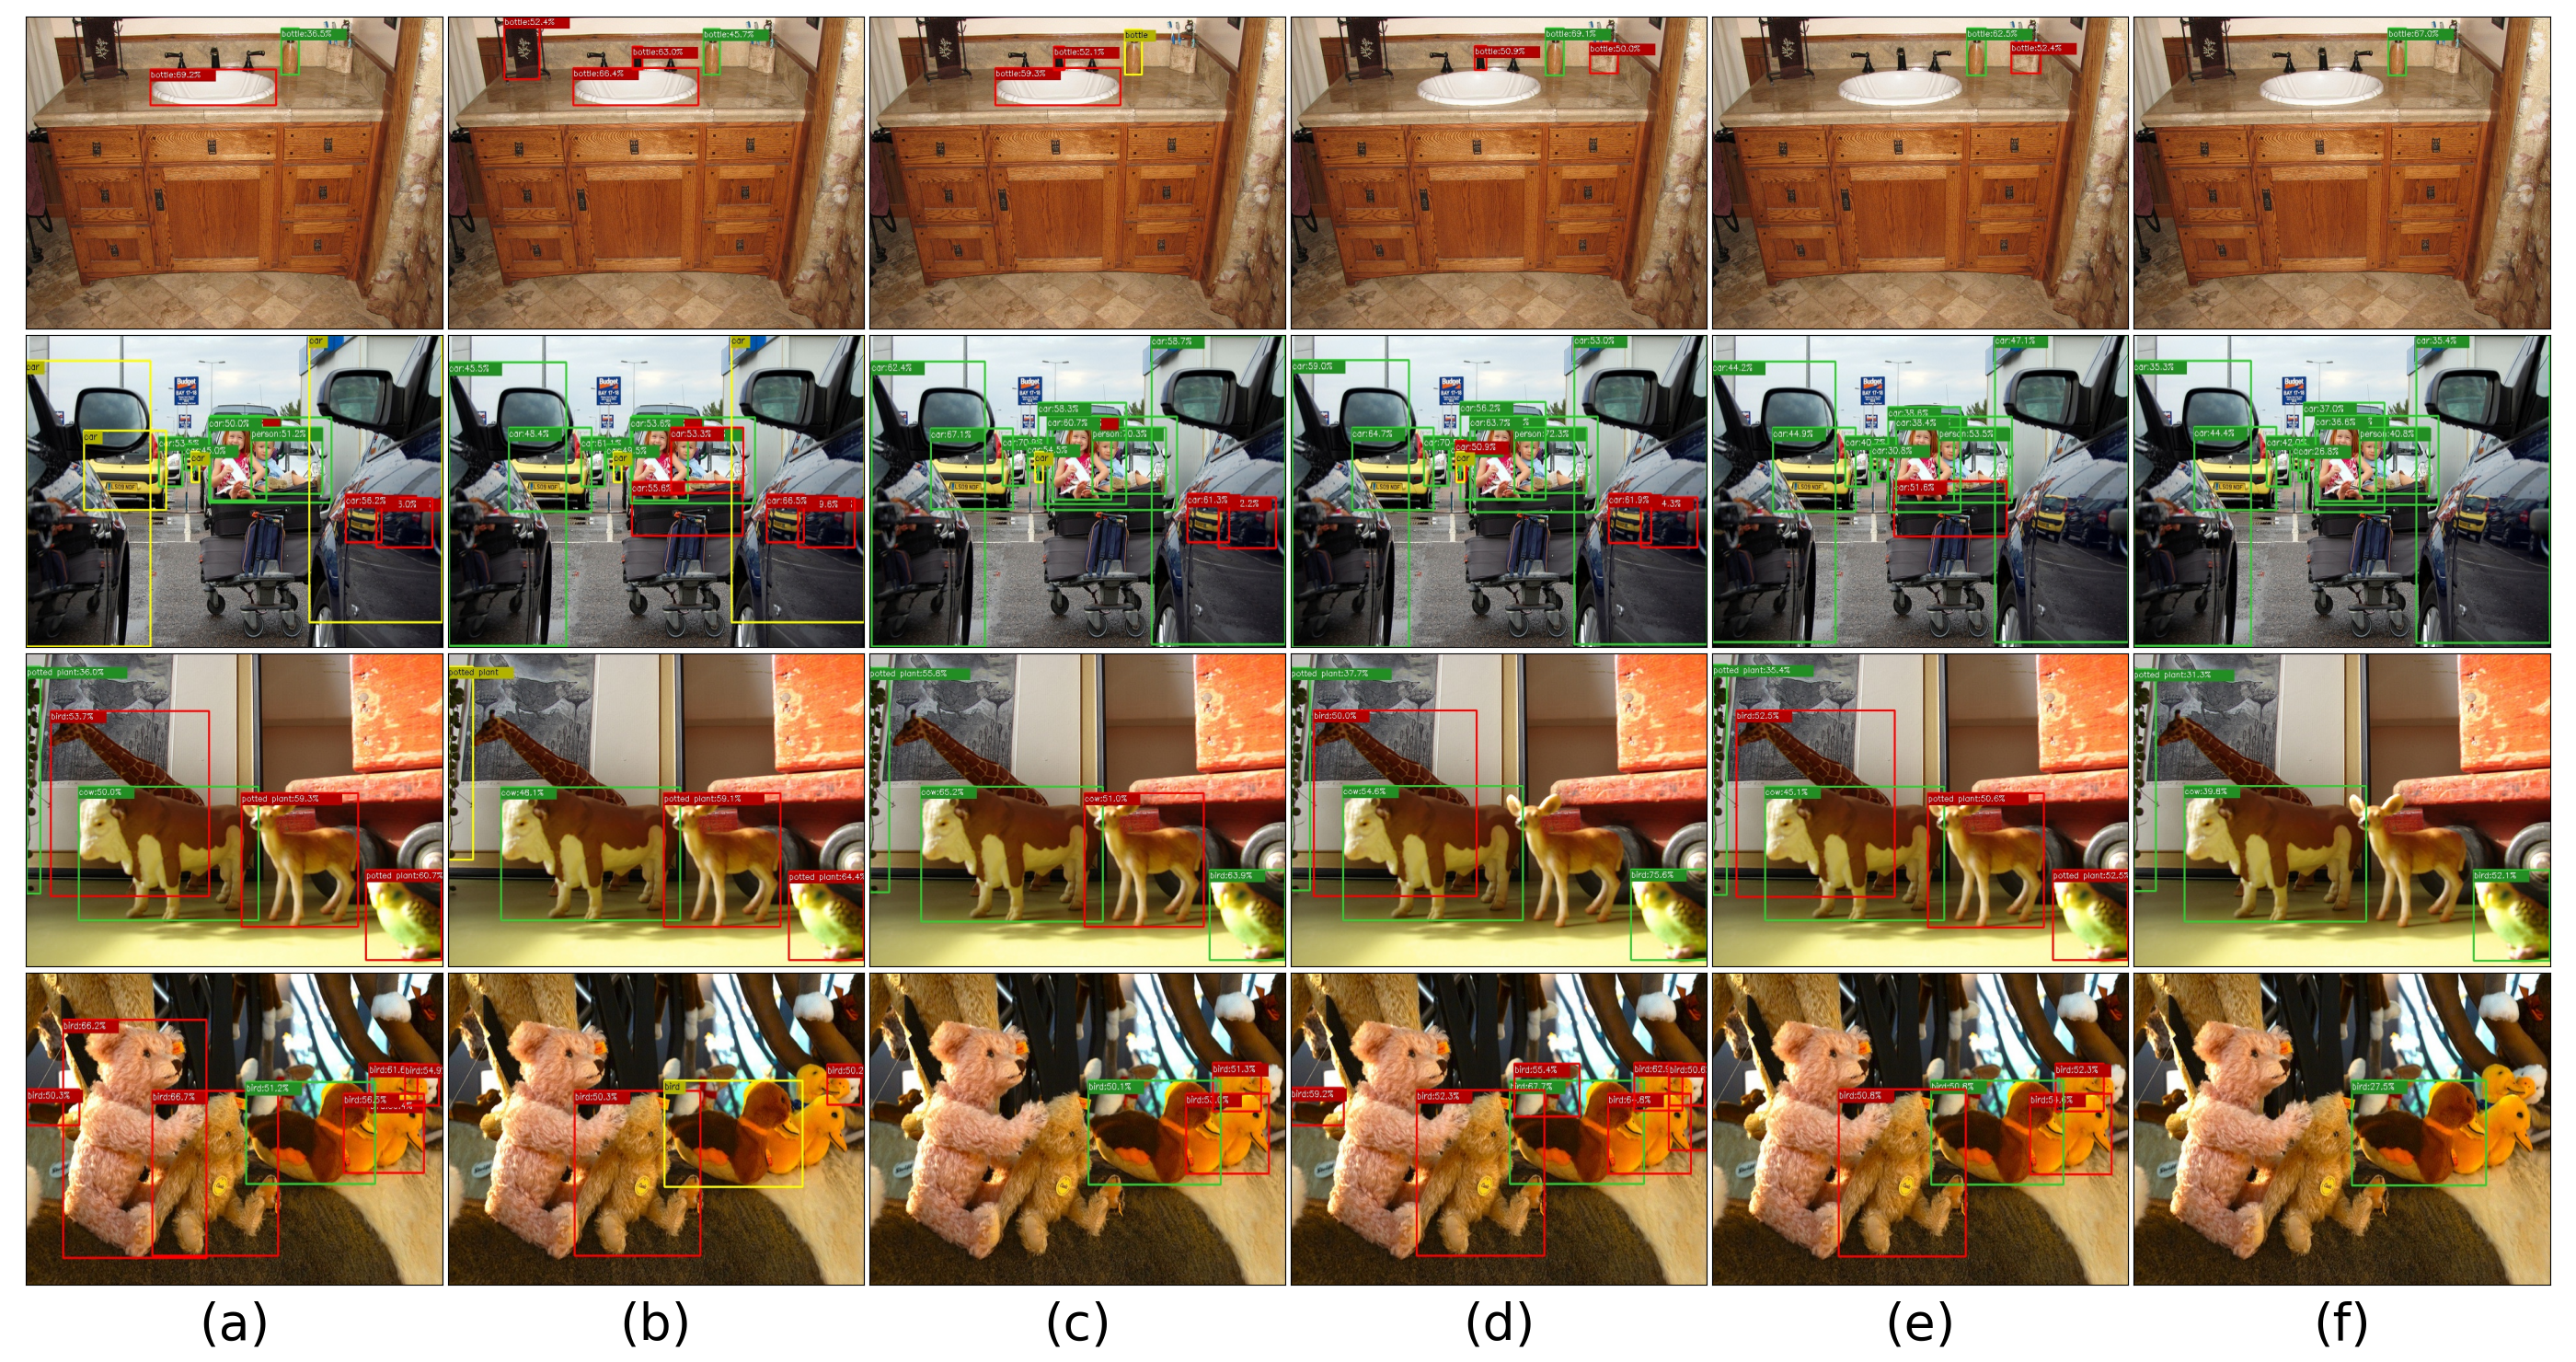
\includegraphics[width=\linewidth]{chapters/PAPERS/VisTex_ICCV_ver/vis_com.png}
  \caption{COCO 上的检测可视化对比。绿/红/黄框分别表示真阳性/假阳性/假阴性。}
  \label{fig:vistex_vis}
\end{figure}


\section{本章小结}
本章提出 VisTex-OVLM，通过视觉文本化将支持图像投影到 OVLM 的文本特征空间，使图像提示能够在不改动 OVLM 主体结构的情况下参与提示推理。借助 MSTB 的多尺度映射与 MSF 的多阶段融合，VisTex-OVLM 在标准少样本基准与开放集迁移设置中均取得了显著提升，验证了“以图像补充文本语义、且保持预训练图文对齐”的有效性。
